\documentclass[11pt]{article}
\usepackage[utf8]{inputenc}

\usepackage{hyperref}
\hypersetup{colorlinks, urlcolor=blue}

\usepackage{tabularx}

\usepackage[margin=1in, head=1in, top=1.5in]{geometry}
\usepackage[parfill]{parskip}

\usepackage{fancyhdr}
\pagestyle{fancy}
\usepackage{graphicx}
\rhead{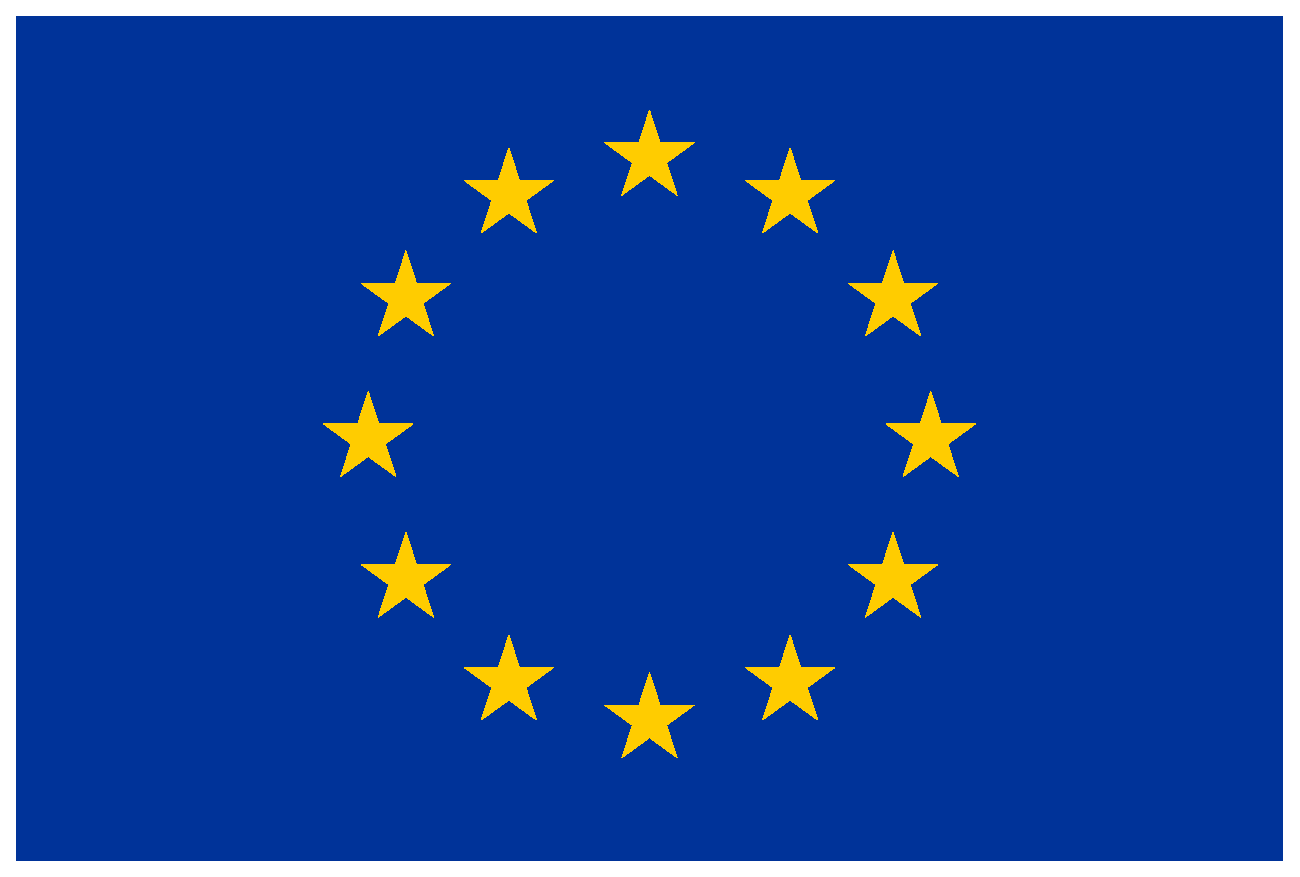
\includegraphics[height=1.5cm]{Flag_of_Europe}}
\chead{\footnotesize\textit{This project has received funding from the EU FP 7 grant number \\ 283883, Horizon 2020 grant agreement No 654000 and Horizon \\ 2020 grant agreement No. 823852.}}
\lhead{
\includegraphics[height=1.5cm]{PaNOSC_cmyk_positivo}}


\begin{document}

\begin{center}
    \section*{DATA PROTECTION INFORMATION IN CONNECTION WITH PAN-LEARNING}
\end{center}

In accordance with the General Data Protection Regulation (hereinafter: GDPR) 2016/679 of the European Parliament and Council, the PaN-Learning team ensures, as set out in the present data protection document, the respect for the principle of transparency and the right of data subjects to be informed in advance and receive clear and comprehensible information on the facts relating to the processing of their personal data in connection with using the services available under the \href{https://pan-learning.org}{https://pan-learning.org}.

Before creating an account (registering) at pan-learning.org, you have to take cognisance of all aspects of the content of the present data processing information in connection with your personal data given by you. By signing up to PaN-learning you certify your acceptance of the present data protection information. 

\subsection{Data controller}
\begin{tabularx}{\textwidth}{@{} X l}
    Name    &  PaN-learning Team (\href{https://pan-learning.org}{https://pan-learning.org})  \\
    Project leader  & Thomas Holm Rod, DRAM group leader, ESS DMSC, Copenhagen \\
    Contact & \href{mailto:admin@pan-learning.org}{admin@pan-learning.org} \\
\end{tabularx}

\subsection{Purpose of data processing}	
Identification of the registered participant of one or several courses on pan-learning.org to allow the participants to have access to the PaN-learning platform. 

\subsection{Scope of processed data}
Personal data given on the enrolment form: first name, last name, e-mail address, requested username, country, institution, field of interest. Note that providing the insitution, country and field of interest are optional. 

\subsection{Access to personal data}
If participants as data subjects are enrolled in one or several courses on pan-learning.org, the designated teachers and students of those courses will see the participants’ enrolment, first and last name.

If participants are enrolled in one or several courses on pan-learning.org, the designated teacher(s) of those courses will have access to track the participants’ progress within the course including attempts and grades in quizzes and will have access to the participants email address. Fellow students will not have access to track participants’ progress including attempts and grades in quizzes or see the participants email address.

The site administrators have access to all personal data given on the enrolment form and have access to track the participants’ progress within courses including attempts and grades in quizzes.

\subsection{Legal ground of data processing}
Consent of the data subject is in accordance with Section 6 (1) Point a) of the GDPR.

\subsection{Time scope of data storage}
Data will be stored until the date when the data subject withdraws his or her consent. As a pan-learning user, data subjects have the right at any time to withdraw their consent by sending a request for removal of their personal data to the following e-mail: \href{mailto:admin@pan-learning.org}{admin@pan-learning.org}.  

\subsection{Data storage method}
Personal data are stored only electronically. 

\section{Enforcement of the rights of data subjects}

\subsection{Right to Information:}
The data subject may request information on the processing of his or her personal data.

A site administator (hereinafter: data controller) shall respond to the request related to the processing of the personal data of the data subject in writing without undue delay and in any event within one month of receipt of the request.

The responce shall cover the information specified in Article 15 (1) of the GDPR, insofar as the information of the data subject cannot be refused by law. The data controller shall take appropriate measures to provide the data subject with all information concerning the processing of personal data referred to in Articles 13 and 14 of the GDPR. Notification in accordance with Articles 15 to 22 and Article 34 of the GDPR shall be provided in a concise, transparent, comprehensible and easily accessible form. The responce shall be provided in writing (e-mail). Oral information may be provided at the request of the data subject, provided that the identity of the data subject has been otherwise established.

The notification is, in principle, free of charge, and the data controller may charge a fee only in the case specified in Article 12 (5) (a) of the GDPR.

The data controller shall reject the request for information only for the reasons specified in Article 12 (5) (b) of the GDPR, and this may only be done in writing, with due justification and appropriate information.

\subsection{Right to Correction and Deletion (right to be forgotten):}
Inaccurate data shall be corrected by the data controller and they shall take steps to delete the processed personal data if the reasons set out in Article 17 of the GDPR exist.

The data subject shall have the right to request the deletion of the personal data concerning him or her without undue delay and the data controller shall delete the personal data concerning him or her without undue delay, in particular if one of the following reasons exists:

\begin{itemize}
    \item personal data are no longer required for the purpose for which they were collected or otherwise processed;
    \item the data subject withdraws his or her consent and there is no other legal basis for the data processing;
    \item the data subject objects to the data processing and there is no overriding legitimate reason for the data processing or the data subject objects to the data processing for the direct acquisition of business;
    \item personal data have been processed unlawfully;
    \item personal data were collected in connection with the provision of information society services to children under the age of 16.
\end{itemize}

If the data controller has disclosed the personal data and the personal data are no longer needed for the purpose for which they were collected or otherwise processed, it shall be deleted and the data controller shall take reasonable steps, taking into account the available technology and implementation costs including technical measures, to inform other controllers that the data subject has requested the deletion of links to, copies or duplicates of the personal data in question. 

\subsection{Right to restriction of data processing:}
In accordance with Article 18 of the GDPR, the data subject has the right to request the data controller to restrict the data processing if
\begin{itemize}
    \item the data subject disputes the accuracy of the personal data (in this case, the restriction applies to the period of time that allows the data controller to verify the accuracy of the personal data);
    \item the processing is unlawful and the data subject opposes the deletion of the data and instead requests that their use be restricted;
    \item the data controller no longer needs personal data for the purpose of data processing, but the data subject requests it in order to submit, enforce or protect legal claims;
    \item the data processing is necessary for the performance of a task in the public interest or the data processing is necessary for the legitimate interests of the data controller or a third party and the data subject has objected to the data processing for these purposes (in this case the restriction takes precedence over the legitimate reasons of the data subject).
\end{itemize}

Restriction of processing means that the data controller does not process the personal data affected by the restriction, except for storage, or only to the extent to which the data subject has consented. The data controller may, in the absence of such consent, handle the data necessary to protect the rights of another natural or legal person or, in the overriding public interest, of the Union or of a Member State of the European Union. 

\subsection{The Right to Data Portability:}
In the course of the data processing activities of the data controller recorded in this present data protection information, no data processing activity is carried out that would require the provision of data portability.

\subsection{Automated Decision Making in Individual Cases, Including Profiling:}
Automated decision-making does not take place during the data Controller's data processing activity described in this present data protection information.

\subsection{Right to Compensation for Damage Caused by Unlawful Data Processing:}
The data controller shall also reimburse the damage caused to others by the unlawful processing of the data subject's data and by the breach of data security requirements, furthermore the damages caused by the personal data breach by the data controller. The data controller shall be released from liability for the damage caused and the obligation to pay damages if he proves that the damage or the violation of the data subject's personal rights was caused by an unavoidable cause outside the scope of data processing. Likewise, it does not compensate for damage if it was caused by the intentional or grossly negligent conduct of the injured party.

\subsection{Right to Legal Remedy:}
The relevant legal remedy or complaint may be addressed by the data subject to the data controller's following e-mail address: \href{mailto:admin@pan-learning.org}{admin@pan-learning.org} directly or to the European Data Protection Board’s e-mail address: \href{mailto:EDPB-DPO@edpb.europa.eu}{EDPB-DPO@edpb.europa.eu}. According to Article 79 of the GDPR proceedings against a data controller shall be brought before the courts of the Member State where the controller has an establishment. Alternatively, such proceedings may be brought before the courts of the Member State where the data subject has his or her habitual residence, unless the controller is a public authority of a Member State acting in the exercise of its public powers.


\end{document}
